%-----------------------------------------------------------------------------
%	 Internet de las Cosas
%-----------------------------------------------------------------------------

\lhead[\thepage]{Internet de las Cosas \thechapter. \rightmark}
\rhead[Internet de las Cosas \leftmark]{\thepage}

%	Capitulo 3: Internet de las Cosas
\chapter{Internet de las Cosas}
\markboth{Internet de las Cosas}{Internet de las Cosas}
\section{Definición}
\lhead[\thepage]{\thesection. Definición}
El ``Internet de las Cosas", también conocido como IoT por sus siglas en inglés es el término utilizado para designar al conjunto de artefactos y dispositivos que poseen la capacidad de conectarse entre ellos o a otras redes como el internet de forma que pueden transmitir y recibir datos e información. De manera formal no existe una definición estandarizada sobre el concepto de IoT, pues dependiendo de la organización puede considerarse el concepto desde el punto de vista desde el cual se observe el concepto, sea desde la perspectiva de las redes, desde el punto de vista de los dispositivos o bien desde el punto de vista de los sistemas automatizados.\\

La primera aparición del término fue realizada en la conferencia ``Congressional Black Caucus Foundation 15th Annual Legislative Weekend'' en Washington, D. C. en septiembre del año 1985 por parte de Peter Lewis \cite{IoTTrueHistory} en donde define que ``El Internet de las cosas, o IoT, es la integración de personas, procesos y tecnología con dispositivos y sensores conectables para permitir el monitoreo, estado, manipulación y evaluación remota de las tendencias de dichos dispositivos''\cite{IoTFirstDef}.\\

Sin embargo este concepto fue olvidado hasta el año 1999 cuando Kevin Ashton independientemente lo utilizó ilustrar el poder de conectar Etiquetas de Identificación por Radio Frecuencia (RFID) usadas en las cadenas de suministro corporativas a Internet para contar y rastrear mercancías sin la necesidad de intervención humana\cite{iotInternetSociety}.\\

Para fines prácticos, durante esta investigación se toma el concepto de original de Peter Lewis, al ser una propuesta genérica e independiente del aspecto funcional examinado. Sin embargo es importante recalcar el hecho que las Las diversas definiciones de IoT no necesariamente están en desacuerdo, sino que enfatizan diferentes aspectos de las tecnologías aplicadas sobre los dispositivos IoT desde diferentes puntos focales y casos de uso\cite{iotInternetSociety}.

\vspace{50px}

\section{Modelos de Comunicación}
\lhead[\thepage]{\thesection. Modelos de Comunicación}
Desde el punto de vista teórico, los dispositivos IoT pueden interconectarse de varias formas. Estos siguen el marco de desarrollo planteado por el estandar RFC-7452\cite{rfc7452} en el que se plantean 4 modelos de comunicación con características propias. Esos modelos son:

\subsection{Comunicación Dispositivo a Dispositivo}
Este modelo de comunicación es el mas simple de todos los paradigmas y consiste básicamente en poder conectar directamente los dispositivos independientemente del medio usado Los dispositivos se comunican usando alguno de los protocolos y estándares disponibles que sean capaces de comprender. En el ámbito del IoT esta comunicación se realiza de manera inalambrica y donde los datos o instrucciones suelen ser bastante pequeños o poco frecuentes (figura \ref{fig:d2d}). En grandes cantidades estaríamos en presencia de un modelo netamente distribuido.
\begin{figure}[htb]
\centering
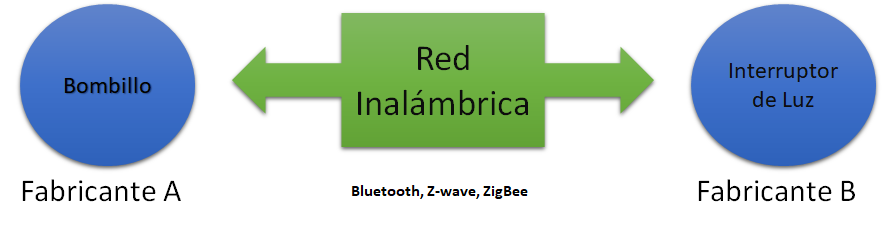
\includegraphics[scale=0.4]{./Figuras/d2d.png}
\caption{Modelo dispositivo a dispositivo}
\label{fig:d2d}
\vspace*{-10pt}
\end{figure}

  
\subsection{Comunicación Dispositivo a la Nube}
En el modelo de comunicación dispositivo a la nube, la conexión del dispositivo se conecta directamente a una nube (propia o federada) usando un proveedor de servicio (figura \ref{fig:d2n}). Este enfoque frecuentemente se aprovecha de los mecanismos de comunicación como redes celulares o la infraestructura de procesamiento de una  organización de manera directa para establecer la conexión entre el dispositivo y el servicio en la nube.
\begin{figure}[htb]
\centering
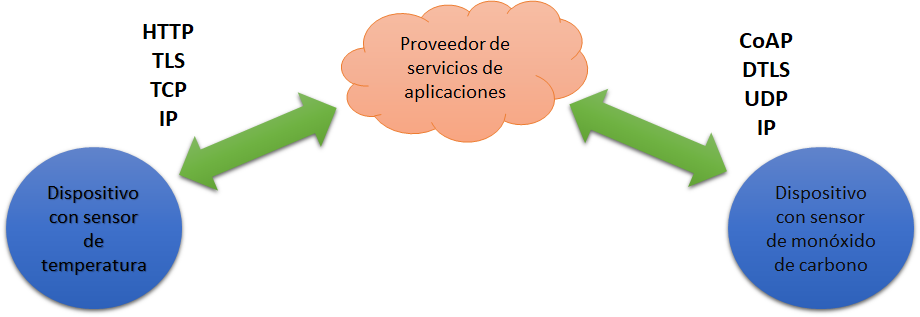
\includegraphics[scale=0.4]{./Figuras/d2n.png}
\caption{Modelo dispositivo a la nube}
\label{fig:d2n}
\vspace*{-10pt}
\end{figure}

\subsection{Comunicación Dispositivo a Puerta de Enlace}
El modelo de comunicación dispositivo a puerta de enlace establece una dispositivo o capa intermedia que concentre todas las comunicaciones (hub o broker) entre los dispositivos y de allí de ser necesario a otros fragmentos de la red o a internet (figura \ref{fig:d2g}). La ventaja de este enfoque es la capacidad de operar de manera centralizada parte de las comunicaciones de los dispositivos. Muchos protocolos están basados en el principio del paradigma de cliente-servidor por lo que este se adapta de manera natural al modelo.
\begin{figure}[htb]
\centering
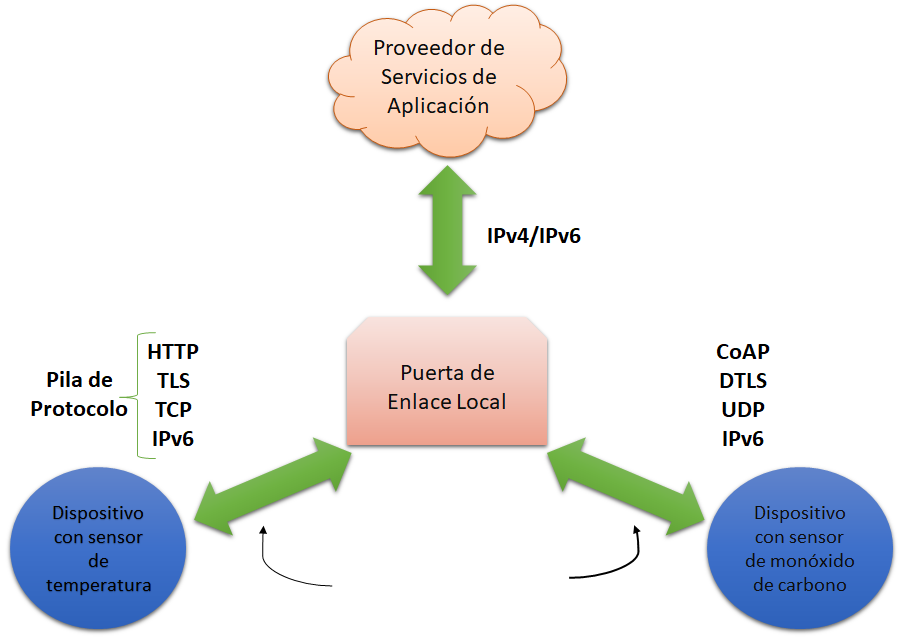
\includegraphics[scale=0.4]{./Figuras/d2g.png}
\caption{Modelo dispositivo a puerta de enlace}
\label{fig:d2g}
\vspace*{-10pt}
\end{figure}

\subsection{Comunicación Dispositivo a Intercambio de Datos en Back-end}
Este modelo es una forma automatizada de conexiones, en donde el dispositivo envía los datos a una o más APIs para de manera transparente, haciendo que este pueda intercambiar la información entre servicios que no necesariamente están estructurados o que pertenecen a un tercero (figura \ref{fig:d2b}). Particularmente este modelo es útil cuando se requiere que la información sea fácilmente accesible a través de múltiples plataformas o sistemas independientes.
\begin{figure}[htb]
\centering
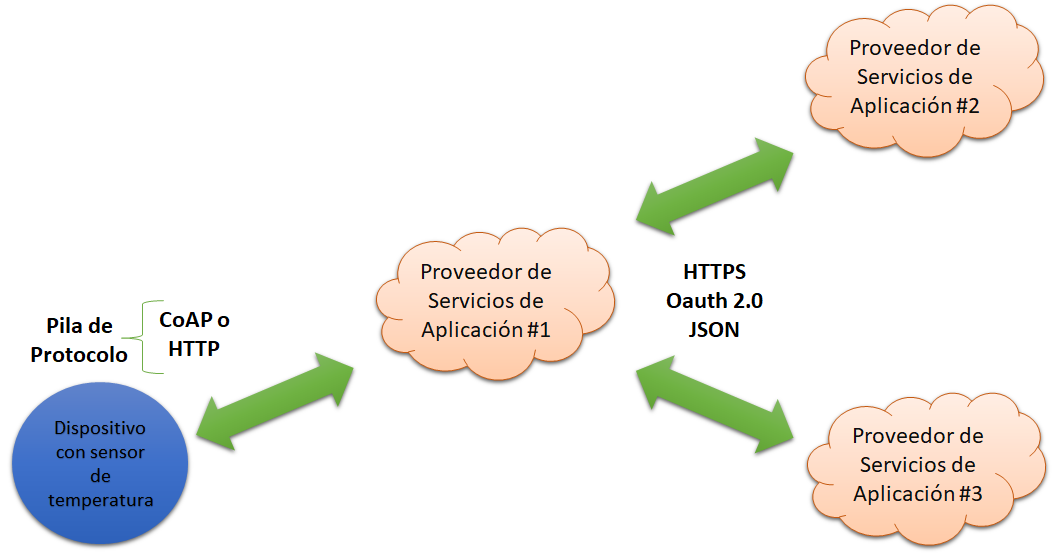
\includegraphics[scale=0.4]{./Figuras/d2b.png}
\caption{Modelo dispositivo a intercambio de datos en back-end}
\label{fig:d2b}
\vspace*{-10pt}
\end{figure}

\section{Aplicaciones del Internet de las Cosas}
\lhead[\thepage]{\thesection. Aplicaciones del Internet de las Cosas}
Si observamos la variedad de dispositivos distintos que encontramos tanto en la vida diaria como si pensamos en términos de los sistemas altamente industrializados, se hace evidente que la cantidad de distintos nichos donde el tener sensores o elementos actuadores hace que muchos procesos se vuelvan tanto dinámicos como reactivos. Las posibilidades de adopción dispositivos interconectados en flujos para automatizar procesos es algo que se está proporcionando la base de lo que llamamos computación ubicua.

Podemos categorizar según las formas de acción y su características, varios campos donde el internet de las cosas tiene y tendrá un impacto significativo para las personas y organizaciones. En la tabla \ref{tabla:categorias_dispositivos} podemos observar alguna de esas categorías y ejemplos de tecnologías acordes\cite{tablaiot}.

\begin{table}[ht]
\centering
\begin{tabular}{| m{3.2cm}| m{4.5cm}| m{6.6cm}|}
\hline
\multicolumn{3}{|c|}{Dispositivos de Internet de las Cosas} \\
\hline 
\centering Uso & \centering Descripción & \centering Ejemplos \tabularnewline \hline
Personas & Dispositivos acareados o implantados en el cuerpo humano & Dispositivos (tecnologías vestibles o digeribles) para monitorear y mantener la salud y el bienestar. Administración de tratamientos, incremento en desempeño del ejercicio físico \\ \hline
Hogar & Casas y edificios & Control de objetos y recursos del hogar y sistemas de seguridad\\ \hline
Ventas & Tiendas y distribuidores a minoristas & Tiendas, bancos, restaurantes, estadios, cualquier lugar donde un consumidor obtenga un producto o un servicio. Ofertas en tiendas, optimización de inventarios \\ \hline
Oficinas & Espacios de trabajo y de generación de conocimiento & Administración de recursos, seguridad en las oficinas. Productividad mejorada \\ \hline
Fabricas & Entornos de producción estandarizados & Lugares donde tengan rutinas repetitivas de trabajo, incluyendo granjas o lineas de producción. Operaciones eficientes, uso de equipamiento optimizado y de inventarios \\ \hline
Lugares de Construcción y extracción de material & Producción de materias primas & Infraestructuras en Minas, Petroleo y gas. Mantenimiento predictivo; seguridad laboral \\ \hline
Vehículos & Sistemas dentro de vehículos & Vehículos incluyendo carros, camiones, barcos, aviones y trenes. Mantenimiento basado en condiciones del sistema. Diseños basados en uso. Analítica preventas \\ \hline
\end{tabular}
\caption{Dispositivos de Internet de las Cosas basados en su campo de uso según McKinsey Global Institute}
\label{tabla:categorias_dispositivos}
\end{table}

\subsection{Hogares}
En los ambientes domésticos, tecnologías como el IoT son de rápida adopción. Ya podemos observar una amplia gama de distintos dispositivos que van desde bombillos inteligentes, pasando por artefactos de linea blanca hasta elementos estructurales como sensores en tuberías que permiten tener un nivel no solo de automatización sobre labores que tradicionalmente son tediosas o difíciles de realizar.\\

Las tecnologías IoT dentro de los hogares permiten tener una amplia posibilidad de personalización y comodidad, ademas que una de las promesas es que al operar obteniendo datos ambientales y de los recursos utilizados puede ajustar y optimizar su utilización lo que representa un nivel de eficiencia que antes no era posible verificar a tan alto detalle. También es posible ahora generar una serie de tareas programadas  o rutinas diarias de los habitantes, que van desde aprovechar la luz solar en las habitaciones, limpieza de robots de las habitaciones o incluso ciertos aspectos de cuidados de mascotas también son posible ahora de administrar gracias a dispositivos inteligentes.\\

Hablando del manejo y monitoreo de recursos también ahora se abre la posibilidad de atender fenómenos recurrentes o críticos. Por ejemplo, sensores en tuberías pueden determinar si el flujo y la calidad de agua es adecuado para el consumo de la vivienda, pero también determinar si existe alguna anormalidad como filtraciones. Otro caso donde puede verse uso son los sistemas de calefacción y aire acondicionados basados en termostatos inteligentes que se adaptan a la temperaturas existentes junto con otros sensores como los de movimientos dentro de una habitación para determinar la exigencia de tener una temperatura adecuada pero teniendo en cuenta el ahorro energético.\\ 

Aspectos como la seguridad también se hacen presentes en esta categoría. Los ya tradicionales sistemas de circuitos cerrados ahora son capaces de orquestarse junto con sensores de movimiento para poder determinar un escenario de intrusión o daños a la propiedad. También mediciones como los niveles de CO2 y otros gases pueden alertar a los interesados sobre condiciones potencialmente peligrosas para los habitantes, incluso con la capacidad de alertar a las autoridades sobre el hecho anormal. 

\subsection{Industrias}
Uno de los sectores con experiencia en la adopción de dispositivos con amplia variedad de sensores y actuadores son las industrias. Desde procesos roboticos cuya tolerancia sea mínima o flujos de tareas criticas para las operaciones  se han aprovechado de esto durante años. Sin embargo la llamada industria 4.0 ahora agrega el factor de la interconexión de los sistemas con los dispositivos para presentar estados e información en tiempo real de los procesos automatizados.\\

Con la información obtenida de todos sensores implicados en los procesos automatizados los gerentes pueden entender de mejor forma se debe proceder a realizar una o mas tareas, ademas de ayudar a optimizar y encontrar puntos de mejorasen  todas las etapas del proceso de producción, desde el suministro, el desarrollo y la creación, ahorrando tiempo y dinero al mismo tiempo\cite{ibmiotindustria}.\\

La retroalimentación que se va generando en las automatizaciones debido a la existencia de estos dispositivos a manera de diagnostico ayudan a poder hacer ajustes de manera inmediata en cadenas de producción y lineas de ensamblaje. Otro aspecto positivo es tener la capacidad de monitoreo y funcionamiento optimo de maquinaria, de forma de realizar mantenimientos preventivos, lo que a la larga representa una reducción de costes y una mejora en la vida útil de las herramientas. 

\subsection{Transporte}
En el caso del transporte, tanto público como privado las oportunidades que representa la capacidad de agregar sensores de manera transversal a la infraestructura existente es uno de los focos que tanto fabricantes, reguladores y gobiernos desean alcanzar. La revolución de los automóviles  con capacidades de conducción autónoma es un ejemplo claro de como los sensores son capaces de brindar los datos necesarios para la toma de decisiones de los sistemas de control del automóvil sin asistencia y esa información recolectada es también útil para entrenar modelos de inteligencia artificial que permitan elevar el nivel de autonomía en la conducción de futuros modelos\cite{ibmiottransporte1}.\\

Otro punto que se benefician es en la cadena de suministros de repuestos. Un medio de transporte que es capaz de diagnosticar anomalías hace posible que se genere una cadena de producción directa a las necesidades requeridas, desde la fabrica de la parte hasta la solicitud de chequeo por parte del usuario.\\ 
 
En los sistemas públicos de transporte se benefician de poder traducir los datos en predicciones y en alertas para los usuarios, para ajustar itinerarios y también para poder masificar los servicios a mas personas, adapatandolo a las necesidades del entorno o del momento.\\

\subsection{Comercio y Logística}
El comercio de bienes y servicios se ajusta a los modelos de intenet de las cosas al tener una observabilidad que no se tenia previamente. Desde sensores que dan estado de un producto desde su producción hasta el momento en que es adquirido y garantizan su calidad hasta datos de localización para la vigilancia de mercancías son tecnologías que ya en la actualidad se utilizan trayendo beneficio a productores como a consumidores en general, haciendo mas transparente la cadenas de producción, buscando eficiencia  y sostenibilidad como factores importantes en la actualidad.\\

Por el lado de la logística el rastreo de bienes, el intercambio de información de inventarios de manera automática basados en la identificación de productos entre proveedores, minoristas y consumidores finales genera confianza y representa nuevo niveles de seguridad, sobre todo al momento de hacer entregas de mercancías.

\subsection{Tecnologías Vestibles}
Los weareables o tecnologías vestibles es uno de esos ámbitos en donde poco a poco se esta encontrando un nicho entre las personas. Desde relojes inteligentes, lentes para realidad aumentada y realidad virtual, prendas de vestir que vigilan nuestros signos vitales, entre otros muchos ejemplos son la forma que el internet de las cosas toma forma para esta categoría. La miniaturización de sensores y de elementos de computo está haciendo posible poder crear dichos elementos y que sean cada vez mas comunes en la vida cotidiana a pesar de retos como el consumo energético de los sensores y de las comunicaciones que estos realizan\cite{ibmappsiot}.\\

Accesorios como relojes inteligentes que son capaces de leer múltiples variables fisiológicas de forma de brindar un panorama general de la salud y otras características personales o trajes especiales, utilizados sobre todo en los deportes donde se busca tener una observación mas marcada del desempeño del deportista los dispositivos ayudan a brindar una mejor perspectiva de cara a entrenamientos y de encontrar métodos para alcanzar mas rendimiento brindando métricas en tiempo real como de forma histórica.

\subsection{Medicina y Salud}
Muy a la par de las tecnologías vestibles, el área de la salud en general se ve beneficiada de la capacidad de poder obtener lecturas de variables fisiológicas así como de los signos vitales que puedan presentar los pacientes  tanto en tiempo real como a lo largo de una intervención o de un tratamiento, así poder adaptar procedimientos, medicinas, dietas de los pacientes en búsqueda de una mas rápida evolución y mejora de las personas.\\

También podemos ver un avance en la efectividad de tratamientos médicos suministrados gracias a la capacidad de obtener la información de manera mas rápida y global por la presencia de esos sensores en los dispositivos que lleven los pacientes, sumando a la tendencia de poder brindar cada vez más tratamientos personalizados \cite{ibmiotmedicina}. Ademas la conectividad del sistema de atención de la salud a través del internet de las cosas, hace hincapié en las necesidades del paciente, es decir, tratamientos proactivos, precisión mejorada cuando se trata de diagnostico, la intervención oportuna por parte del personal de salud, en miras de una medicina cada vez mas preventiva en vez de una que sea reactiva. 

\subsection{Ciudades Inteligentes}
Las ciudades en el futuro se perfilan en el uso de los dispositivos IoT como parte fundamental de la infraestructura que deben tener para brindar a sus ciudadanos la mayor cantidad de satisfacción y calidad de vida posible. Desde el punto ya tocado del transporte como el monitoreo y control de recursos vitales como es el caso del acceso a agua potable, el reciclaje de materiales, los gobiernos ya diseñan en función de la capacidad de poder contar con data de sensores para poder evaluar mejores políticas ciudadanas, así como también brindar transparencia a los procesos de gestion de recursos\cite{ibmiotciudad}. 

\section{Interoperatividad entre Infraestructuras y Dispositivos}
\lhead[\thepage]{\thesection. Interoperatividad entre Infraestructuras y Dispositivos}
Para las redes de computadoras, la interoperatividad es un elemento fundamental, incluso desde su mismo diseño, pues la idea de dispositivos conectados también requiere que se puedan comprender en un ``lenguaje" común entre las partes. Para ello existen numerosos estándares y protocolos que han surgido de forma que sean ese marco común de entendimiento entre plataformas, dispositivos y arquitecturas.\\

Más allá de los aspectos técnicos, la interoperatividad tiene una influencia significativa en el impacto económico potencial de IoT. Aquellos marcos comunes, estándares y protocolos que tienen bien definido pueden fomentar la innovación y proporcionar a los fabricantes de dispositivos IoT valor agregado gracias a esas características y a su vez, aumentar el valor económico general del mercado.\\

Además, la aplicación de las normativas y el desarrollo de nuevos estándares abiertos, cuando sea necesario, ayudan a reducir las barreras de entrada, facilitan nuevos modelos de negocio y se convierten en opciones para el usuario final así como a las organizaciones quienes las regulan o las usan. Facilita la posibilidad de elegir dispositivos con las mejores características al mejor precio e integrarlos para que trabajen juntos. Los compradores pueden ser reacios a adquirir productos y servicios IoT si hay inflexibilidad en la integración, alta complejidad de uso, la propiedad final de información obtenida o la preocupación por el bloqueo del proveedor o temor a la obsolescencia debido al cambio de los estándares\cite{iotInternetSociety}.\\

\subsection{Ecosistemas}
Los ecosistemas de dispositivos IoT no son más que la consideración planificada bajo el paraguas de uno o más estándares y/o protocolos para ofrecer características que den al usuario final un valor sobre su elección. Existen dos perspectivas sobe los ecosistemas de los dispositivos: 
\begin{itemize}
\item Ecosistemas abiertos: Generalmente creados por una organización bajo el apoyo de múltiples empresas u otras organizaciones con la idea de acordar métodos de operación que sean estandarizados a nivel de las partes interesadas. En el mundo del internet de las cosas se ve bajo la serie de tecnologías y protocolos que han sido adaptados y propuestos para poder realizar desde las tareas de comunicación, así como también en las características que sensores y actuadores envían, procesan y almacenan la información. De propósito libre y con un esquema en el cual los aportes de las comunidades y personas son escuchados tienen un ciclo de desarrollo muy rápido y una alta adopción por su flexibilidad. El principal problema que posee este enfoque es que los esfuerzos de estandarizar o el interés de organizaciones por sobre otras de utilizar las características  de un protocolo o estándar pueden dispersar los esfuerzos de adopción de fabricantes por la cantidad de posibilidades necesarias para validar un funcionamiento correcto de los dispositivos ante múltiples protocolos o estándares y el costo que conlleva. 
\item Jardines mallados: De manera contraria a los ecosistemas abiertos, los jardines mallados son desarrollados por las organizaciones para poder controlar de manera cercana la visión de los estándares y protocolos para el funcionamiento de los dispositivos. Esta visión permite que exista una integración vertical amplia y a su vez, se beneficia de un manejo muy optimo de los recursos disponibles para las tareas relacionadas. Así todos los dispositivos que están certificados para funcionar dentro de un ecosistema de estas características probablemente funcione de una manera mucho mejor de lo que lo haría en un ecosistema abierto. La contra de este enfoque es la poca flexibilidad tanto de fabricantes como de los usuarios finales para obtener características que den valor agregado a los dispositivos que desea obtener\cite{iotInternetSociety}. Ademas es común que los procesos de certificación y el coste de licenciamiento de dichos estándares y protocolos cerrados se traduzca en un precio mayor tanto para los fabricantes como para los usuarios finales.
\end{itemize}

\subsection{Riesgos}
Con respecto al tema de riesgos, podemos separarlos en dos espacios:
\begin{itemize}
\item Riesgos Programados: Los riesgos programados son aquellos riesgos que asumen los fabricantes, empresas y organizaciones al momento de diseñar, crear y ofrecer al publico un producto. En el ámbito del internet de las cosas este riesgo viene por la decisión de tomar uno o más estándares en búsqueda de interoperatividad. También se puede representar por el hecho de que se busque poner en el mercado un producto que no cumpla completamente un estándar con la probabilidad de no poder operar correctamente en un ecosistema.
\item Riesgos Técnicos: Los riesgos técnicos van presentes en las consideraciones de diseños, arquitectura y finalmente la producción de los dispositivos en si mismos. La complejidad del funcionamiento de una o más características puede verse afectada si en algunos de esas etapas existe un fallo o también por algún defecto en los componentes 
\end{itemize}

\subsection{Sistemas Heredados}
Una arista de la interoperatividad que debe considerarse en todo momento tanto como por los fabricantes, como por los usuarios finales es la capacidad de lidiar con sistemas antiguos, también llamados heredados o legados. Esto se debe a que aunque existan estándares y protocolos que son suficientemente robustos pero no están diseñados con la idea de ser extendidos hacen que dispositivos que lleven esos estándares tengan dificultades para poder cumplir con las expectativas de las industrias. Del otro lado, el tener que crear dispositivos nuevos que tengan que cumplir con estándares y protocolos desactualizados puede hacer que los costes sean mayores, así como la dificultad de brindar soporte a los mismos. 

\subsection{Configuración de dispositivos}
La configuración de dispositivos es un proceso que muchas veces es similar en aspectos como la parte de la conectividad. Sin embargo el problema se puede observar cuando la cantidad de dispositivos a configurar es alto. Esta perspectiva puede ser desalentadora para los usuarios finales quienes tienen que asumir el tiempo para hacerlo o el coste de contratación de profesionales para poder realizar todo el proceso. 

\section{Protocolos y Estándares Utilizados}
\lhead[\thepage]{\thesection. Protocolos y Estándares Utilizados}
Como se pudo observar en los puntos anteriores la existencia de estándares y de protocolos son parte fundamental para garantizar el correcto funcionamiento de cualquier dispositivo que entre dentro de cualquiera de las categorías del internet de las cosas. El lado de manejo de las redes como pilar de la tecnología requiere conocer y elegir el método adecuado de comunicarse. Es por ello que tanto los modelos planteados al principio de este capitulo\cite{rfc7452} como el protocolo adecuado puede cambiar diametralmente el desempeño del dispositivo.\\

Sin embargo, hay un valor considerable en la extensión de la capacidad de conectarse a internet a los dispositivos más restringidos en termino de recursos que a menudo necesitan versiones optimizadas o uso especial de estos protocolos. A continuación se presentan algunos de los protocolos y estándares actuales mas importantes empleados por los dispositivos del Internet de las Cosas y que han sido considerados para la investigación y el desarrollo de este trabajo.

\subsection{Protocolos}
\subsubsection{HTTP}
El protocolo de transferencia de hipertexto o mejor conocido como HTTP, es un protocolo de la capa de aplicación para la trasmisión de documentos hipermedia, como HTML. Fue diseñado para la comunicación entre los navegadores y servidores web, aunque puede ser utilizado para otros propósitos también. Sigue el patrón modelo-vista-controlador, en el que se establece una conexión, realizando una petición a un servidor y espera una respuesta del mismo. Se trata de un protocolo sin estado, lo que significa que el servidor no guarda ningún dato (estado) entre dos peticiones. Aunque la mayoría de los casos se basa en una conexión del tipo TCP /IP, pude usarse con cualquier otro protocolo del nivel de la capa de transporte orientado a conexión.\cite{mozillahttp}\\

Las principales características clave del protocolo son las siguiente:
\begin{itemize}
\item Sencillez: HTTP esta pensado y desarrollado para ser leído y fácilmente interpretado por las personas, haciendo de esta manera más fácil la depuración de errores, y reduciendo la curva de aprendizaje para las personan que empieza a trabajar con él.
\item Extensible: Presentadas en la versión HTTP/1.0, las cabeceras de HTTP, han hecho que este protocolo sea fácil de ampliar y de experimentar con él. Funcionalidades nuevas pueden desarrollarse, sin más que un cliente y su servidor, comprendan la misma semántica sobre las cabeceras de HTTP.
\item Basado en sesiones, sin estados: HTTP es un protocolo sin estado, es decir, no guarda ningún dato entre dos peticiones en la misma sesión. Esto plante la problemática, en casó de que los usuarios requieran interactuar con determinadas páginas Web, de forma ordenada y coherente. Pero mientras HTTP ciertamente es un protocolo sin estado, el uso de HTTP cookies, si permite guardar datos con respecto a la sesión de comunicación. Usando la capacidad de ampliación del protocolo HTTP, las cookies permiten crear un contexto común para cada sesión de comunicación.
\item Orientado a Conexión: Una conexión se gestiona al nivel de la capa de trasporte, y por tanto queda fuera del alcance del protocolo HTTP. Aún con este factor, HTTP no necesita que el protocolo que lo sustenta mantenga una conexión continua entre los participantes en la comunicación, solamente necesita que sea un protocolo fiable, o que no pierda mensajes (como mínimo, en todo caso, un protocolo que sea capaz de detectar que se ha pedido un mensaje y reporte un error).
\end{itemize}

HTTP es un protocolo que funciona en dos fases fundamentales, una fase de petición y una fase de respuesta. Esto se hace de la siguiente manera:

\begin{itemize}
\item En la fase de petición:
\begin{enumerate}
\item Se abre una conexión: Se utiliza un protocolo de conexión, generalmente TCP, que se usará para hacer una o una serie de peticiones y recibir una respuesta. El cliente puede abrir una conexión nueva, reusar una existente, o abrir varias a la vez hacia el servidor.
\item Se hace una petición HTTP:  Los mensajes HTTP (previos a HTTP/2) son legibles en texto plano. A partir de la versión del protocolo HTTP/2, los mensajes se encapsulan en franjas, haciendo que no sean directamente interpretables, aunque el principio de operación es el mismo.
\end{enumerate}
\item En la fase de respuesta:
\begin{enumerate}
\item Se recibe y lee la respuesta enviada por el servidor.
\item Se cierra o recicla la conexión para futuras peticiones. 
\end{enumerate}
\end{itemize}

Existen dos tipos de mensajes HTTP: peticiones y respuestas, cada uno sigue su propio formato.

\begin{itemize}
\item Petición HTTP: Consta de un método, que generalmente un verbo como GET o POST que define la operación que el cliente desea realizar, la dirección del recurso pedido en formato de URL, la versión del protocolo y el cuerpo del mensaje. Opcionalmente puede llevar cabeceras que pueden aportar mas información. 

\begin{figure}[ht]
\centering
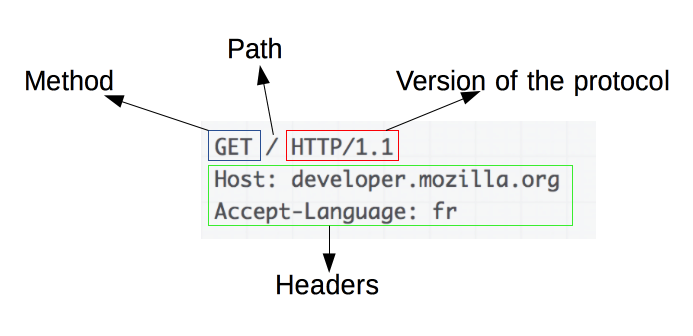
\includegraphics[width=0.625\textwidth]{Figuras/HTTP_Request.png}
\caption{\label{fig:httprequest}Formato de un mensaje de petición HTTP}
\vspace*{-15pt}
\end{figure}

\item Respuesta HTTP: Formados por los campos de versión del protocolo, el código del estado indicando si la petición fue exitosa o no y el porque, una descripción del estado, cabeceras HTTP y por ultimo y dependiendo de lo requerido, un recurso.

\begin{figure}[ht]
\centering
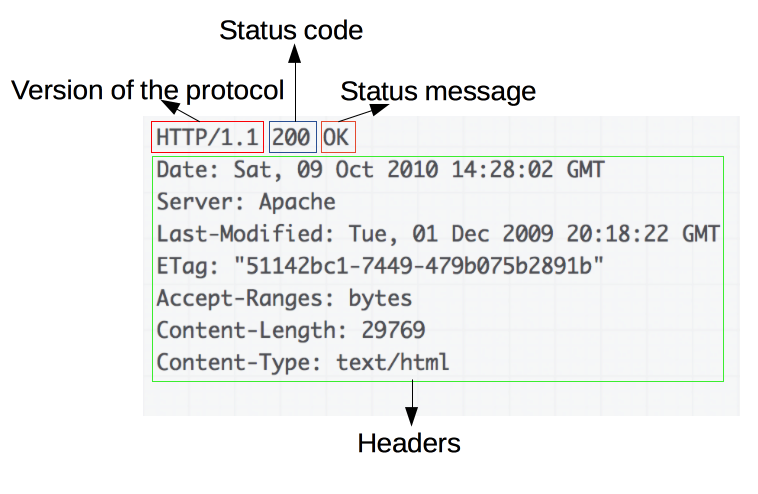
\includegraphics[width=0.5\textwidth]{Figuras/HTTP_Response.png}
\caption{\label{fig:httpresponse}Formato de un mensaje de respuesta HTTP}
\vspace*{-15pt}
\end{figure}

\end{itemize}

\subsubsection{MQTT}
MQTT son las siglas de Message Queue Telemetry Transport. Como su nombre indica, su propósito principal es la telemetría, o el monitoreo remoto. Su objetivo es recopilar datos de muchos dispositivos y transportarlos a la infraestructura de se servicios en red. Se dirige a grandes redes de pequeños dispositivos que necesitan ser monitoreados o controlados desde la nube.\cite{iotprotocols}\\

IBM creo el protocolo MQTT para poder establecer comunicación vía satélite con sensores en campos petroleros. Fue diseñado para que las comunicaciones a través de este protocolo fuesen confiables y utilizando la menor cantidad de energía posible. MQTT utiliza un modelo de publicación-suscripción y requiere un corredor MQTT central (Broker) para administrar y enrutar mensajes entre los nodos de una red MQTT. Utiliza TCP en la capa transporte, que se caracteriza por ser confiable, ordenado y con comprobación de errores.\cite{iotprocolslinkedin}\\

\begin{figure}[ht]
\centering
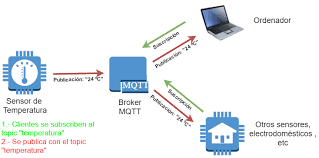
\includegraphics[width=0.85\textwidth]{./Figuras/mqtt.png}
\caption{\label{fig:mqttprotocol}Diagrama de funcionamiento del protocolo MQTT}
\vspace*{-10pt}
\end{figure}

El protocolo MQTT tiene como fortalezas:
\begin{itemize}
\item Modelo de publicación-suscripción: El modelo de publicación-suscripción es un modelo que no tiene problemas al escalar la cantidad de nodos en la red y ademas hace hace de un uso eficiente de la energía. Los Brokers y los nodos publican información y otros se suscriben según el contenido, el tipo o el tema del mensaje. (Estos son términos estándar de MQTT.) Generalmente, el Broker se suscribe a todos los mensajes y luego administra el flujo de información a sus nodos.
\item Seguridad: Al utilizar TCP como protocolo en la capa de transporte, Los paquetes MQTT no están encriptados por defecto. Pero puede utilizar la seguridad de Internet TLS/SSL. TLS es un método muy seguro para cifrar el tráfico, pero también es un recurso intensivo para clientes ligeros debido a su apretón de manos requerido y el aumento del overhead de los paquetes. Para las redes donde la energía es una prioridad muy alta y la seguridad mucho menos, cifrar sólo la carga útil del paquete puede ser suficiente.
\item Soporte para Calidad de Servicio (QoS): En MQTT, los niveles QoS 0, 1 y 2 describen niveles crecientes de entrega garantizada de mensajes. EL nivel 0 no repite paquetes, es decir, es un nivel de ``apunta y dispara". El nivel 1 intenta garantizar que un mensaje sea recibido al menos una vez por el destinatario previsto. Una vez que un mensaje publicado es recibido y comprendido por el destinatario deseado, reconoce el mensaje con un mensaje de acuse de recibo (PUBACK) dirigido al nodo de publicación. Por ultimo el nivel 2 intenta garantizar que el mensaje sea recibido y descodificado por el destinatario deseado. Este es el nivel de QoS MQTT más seguro y confiable. 
\item Testamento y ultima voluntad (LWT): MQTT proporciona un mensaje de ``último testamento" que se puede almacenar en el Broker MQTT en caso de que un nodo se desconecte inesperadamente de la red. Este LWT conserva el estado y propósito del nodo, incluyendo los tipos de comandos que publicó y sus suscripciones. Si el nodo desaparece, el intermediario notifica a todos los suscriptores del LWT del nodo. Y si el nodo vuelve, el corredor lo notifica de su estado anterior. Esta característica acomoda redes con alto porcentaje o probabilidades de  pérdidas.
\item Suscripciones flexibles de temas: Un nodo MQTT puede suscribirse a todos los mensajes dentro de una funcionalidad determinada. Por ejemplo, en un cocina un nodo horno puede suscribirse a todos los mensajes de ``cocina/horno/+", con el ``+" como comodín. Esto permite una cantidad mínima de código. Hay otros comodines MQTT igualmente útiles para reducir la cantidad del código utilizado y por lo tanto el tamaño y el coste de la memoria.
\end{itemize}

Por otro lado MQTT tiene tres desventajas evidentes:
\begin{itemize}
\item El Broker: Como intermediario central puede ser un inconveniente para los sistemas IoT distribuidos. En entornos donde la existe poca presencia de sensores y/o actuadores o donde no crece la cantidad de los dispositivos, la presencia de un Broker general latencia dentro de la red. Por otro lado el Broker puede convertirse en un único punto de fallo para la red completa.
\item El uso de TCP: TCP fue diseñado originalmente para dispositivos con más memoria y recursos de procesamiento que los que pueden estar disponibles en una red de dispositivos IoT. Por ejemplo, el protocolo TCP requiere que las conexiones se establezcan en un proceso de apretón de manos de varios pasos antes de intercambiar cualquier mensaje. Esto aumenta los tiempos de activación y de comunicación y reduce la duración de la batería a largo plazo.
\item Retrasos en la transmisión: Una vez más, el uso de TCP sin persistencia de sesión puede requerir un tiempo de transmisión incremental para el establecimiento de la conexión. Para nodos con tráfico periódico y repetitivo, esto puede afectar el consumo energético.
\end{itemize}

\begin{figure}[ht]
\centering
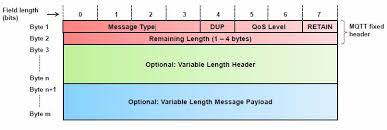
\includegraphics[width=0.9\textwidth]{./Figuras/mqtt_header.jpeg}
\caption{\label{fig:mqttheader}Formato de mensaje del protocolo MQTT}
\vspace*{-10pt}
\end{figure}


\subsubsection{IPv4 e IPv6}
Internet Protocol o IP es un protocolo de capa de red , no orientado a conexión, con una política de mejor esfuerzo en la entrega de los paquetes y cuya principal tarea es permitir la comunicación bidireccional en la red haciendo uso de direcciones a las cuales se pueden enrutar convenientemente. IP no provee ningún mecanismo para determinar si un paquete alcanza o no su destino y únicamente proporciona seguridad (mediante checksums o sumas de comprobación) de sus cabeceras y no de los datos transmitidos. \\

Este protocolo tiene como pilares fundamentales:
\begin{itemize}
\item El direccionamiento: Se refiere a la capacidad de poder asignar una dirección lógica a una interfaz de red y a su ves conocer  la manera en que se divide la red a la que pertenece.  Para el direccionamiento efectivo, el protocolo hace uso de direcciones IP, un sistema de identificación lógica y jerarquicamente una interfaz de red.
\item EL enrutamiento: el enrutamiento permite redistribuir de manera eficiente el trafico de las comunicaciones entre nodos de manera que estos puedan ir de su origen a su destino.
\end{itemize}
 
El protocolo IP en la actualidad conviven dos versiones del protocolo, IPv4 establecido en el RFC-791\cite{rfc791} e IPv6 establecida en el RFC-2460\cite{rfc2460}, ambos basados en los mismos principios pero con diferencias en la implementación.

\subsection{Estándares}
\subsubsection{Bluetooth}
Bluetooth es uno de los primeros estándares de comunicación creados pensando en dispositivos móviles. Desarrollado por la compañía sueca Ericsson estableció un protocolo de comunicación inalambrica en áreas personal, con una tasa de transmisión inicial de 1 Mbps, que luego paso a ser parte del estándar IEEE 802.15.1\cite{ieeebluetooth}. Los dispositivos Bluetooth utilizan señales de radio en la frecuencia de 2.4 GHz para establecer dicha conexión.  Con este estándar se busca que los dispositivos puedan:
\begin{itemize}
\item Establecer conexiones con poco gasto energético.
\item Establecer enlaces por lo general de corta duración.
\item Otorgar seguridad mediante diversas maneras de cifrado de datos, además de exigir el uso de un PIN para establecer conexiones entre equipos.
\item Soportar trafico de voz y datos.
\item Tener un bajo costo de producción e implementación.
\end{itemize}
En la actualidad el estándar Bluetooth se compone de un núcleo o también llamado Bluetooth Core que contiene las directivas de comunicaciones generales e inherentes al estándar y de dos extensiones llamadas Bluetooth BR/EDR (Basic Rate/Enhanced Data Rate) optimizado para hacer uso de intercambio de streams de datos, como audio y el Bluetooth Low Energy diseñado para hacer un uso muy eficiente de la energía utilizada en la comunicación, en casos donde el intercambio de datos es pequeño y que ha sido implementado desde la versión 4.0 del estándar. Los dispositivos tiene la posibilidad de implementar ya sea Bluetooth BR/EDR o Bluetooth Low Energy o ambas de forma mixta.\\

La gran ventaja de este estándar es que gran cantidad de dispositivos cuentan con la capacidad de comunicarse a través de este estándar, ademas de que permite una comunicación con un modelo dispositivo a dispositivo fácil de establecer para el usuario final. Sin embargo estas comunicaciones son de corto alcance cosa que puede afectar el desempeño entre dispositivos. El Bluetooth Low Energy abre las puertas a dispositivos que requieren manejar de manera eficiente el consumo energético de las comunicaciones pero no es aconsejado uso para el intercambio exhaustivo de información. Por otro lado, es recomendable utilizar el Bluetooth BR/EDR cuando la aplicación que se usa requiere enviar una cantidad de información importante o continuamente, pero tiene la desventaja que el consumo energético es mayor afectando negativamente la duración de los dispositivos si estos operan con una fuente estable de energía.

\subsubsection{Redes Celulares}
Los estandares celulares son las mas utilizadas en cuanto a redes inalambricas. Extendidas al rededor del mundo proveen a los dispositivos una manera sencilla de poder conectarse a servicios de voz y datos. \\

Las tecnologías de 3G son la respuesta a la especificación IMT-2000 de la Unión Internacional de Telecomunicaciones\cite{itu2000}. En Europa y Japón se seleccionó el estándar UMTS (Universal Mobile Telecommunication System)\cite{umts}, basado en la tecnología W-CDMA\cite{wcdma}. UMTS está gestionado por la organización 3GPP, también responsable de GSM, GPRS y EDGE. Para el continente americano, para África y para el resto del mundo se establecieron los estándares High-Speed Packet Access (HSPA)\cite{hspa} es una fusión de dos protocolos móviles, High Speed Downlink Packet Access (HSDPA)\cite{hspa} y High Speed Uplink Packet Access (HSUPA)\cite{hspa} que extiende y mejora el rendimiento de las redes de telecomunicaciones móviles de tercera generación (3G), como son el 3.5G o HSDPA y 3.5G Plus, 3.75G o HSUPA existentes utilizando los protocolos WCDMA.\\

La cuarta generación de tecnología en telecomunicaciones móviles, abreviado comúnmente como 4G, es el estándar aplicado al mercado móvil de la actualidad. Para que una tecnología pueda ser considerada como parte del 4G, esta debe de cumplir con ciertos requisitos para ser considerado dentro del estándar. Entre las tecnologías que se encuentran dentro de dicho estándar están: LTE-Advanced\cite{LTE-advanced}, WiMAX móvil(IEEE 802.16e)\cite{ieee80216} y WiMAX Release 2 (IEEE 802.16m).\cite{ieee80216}\\

Los requerimientos para que una red sea considerada 4G  están expuestos en la IMT-advanced de la ITU y son:
\begin{itemize}
\item Alto grado de uniformidad de funciones en todo el mundo, manteniendo al mismo tiempo la flexibilidad de admitir una amplia gama de servicios y aplicaciones rentables.
\item Compatibilidad de servicios con las IMT y las redes fijas.
\item Interoperatibilidad con otros sistemas de acceso radioeléctrico.
\item Servicios móviles con soporte para calidad de servicio.
\item Capacidad de itinerancia mundial.
\item velocidades de 100 Mbits para una movilidad alta y de 1 Gbits para una movilidad baja.
\end{itemize}

Plenamente diseñados para hacer su uso en dispositivos de carácter móvil y aprovechando la infraestructura existente, hacen de los estándares de comunicación celular una de las opciones mas fáciles y convenientes de implementar en soluciones de comunicación inalambrica, sobre todo cuando no se puede implementar una red dedicada para el trafico de los nodos. Hacen un uso eficiente de la energía del dispositivo pues los celulares y teléfonos inteligentes, pues es el recurso critico para las operaciones.

\subsubsection{NFC}
La Comunicación de Campo Cercano o NFC  por sus siglas en inglés, es un estándar que permite transferencia bidireccional de datos entre dispositivos. Su rango de transmisión es corto de máximo 10 cm de distancia, con tasas de transferencia máxima de 420kbps. El conjunto de tecnologías que permiten está comunicación están enmarcados en el estándar ISO/IEC 18000-3.\cite{isonfc}\\

NFC puede funcionar en dos modos:
\begin{itemize}
\item Activo, en el que ambos equipos con chip NFC generan un campo electromagnético e intercambian datos.
\item Pasivo, en el que solo hay un dispositivo activo y el otro aprovecha ese campo para intercambiar la información.
\end{itemize}

En cuanto a la seguridad, NFC utiliza su corta distancia de transmisión como un mecanismo de protección pues cualquier ataque deberá realizarse cerca de los dispositivos que realizan la transmisión. 

\subsubsection{Wifi (802.11)} 
WiFi es el estándar de comunicación inalambrico mas utilizado en el mundo después de las redes celulares y ha sido una selección obvia al momento de integrar comunicación dispositivos con una red. El estándar WiFI esta basado en el estadar de la IEEE 802.11\cite{ieee80211} y ha atravesado una serie de versiones que han permitido mejorar su cualidades de despliegue en termino de distancia, velocidad de transmisión, seguridad e interoperatividad.\\  

El estándar 802.11 consta de una serie de técnicas de modulación half duplex inalambrica que utilizan el mismo protocolo básico. Las versiones 802.11b y 802.11g utilizan la banda ISM de 2,4 GHz. La dificultad que representar esta banda es que los dispositivos pueden sufrir interferencias con electrodomésticos tan comunes como el microondas o el horno o con dispositivos Bluetooth. Es por que eso que deben controlar dicha susceptibilidad a las interferencias mediante métodos de señalización de espectro ensanchado por secuencia directa (DSSS) y de multiplexación por división de frecuencia ortogonal (OFDM), respectivamente.\\

Por otro lado la versión 802.11a y la versión 802.11ac utilizan la banda de 5 GHz. También hay versiones que pueden usar ambas bandas, como 802.11n pueden utilizar las bandas de 2,4 GHz o la de 5 GHz. El alcance de este estandar depende de la potencia del dispositivo, de la versión de WiFi y de las bandas utilizadas, al igual que la velocidad de transmisión pudiendo pasar de 54 Mbps a 1 Gbps. \\

A pesar de ser uno de los estándares mas utilizados, WiFI posee como inconvenientes la complejidad del hardware y software requerido así como también la cantidad de energía requerida para  establecer y mantener la comunicación, convirtiéndose en prohibitivo para dispositivos con capacidades limitadas. En las revisiones mas nuevas del estándar se esta buscando  la manera de que se mantengan las ventajas de transmisión y de espectros utilizados, sin que esto signifique un impacto severo en el consumo energético de los dispositivos. 

\subsubsection{Zigbee}
Zigbee es otro estándar de comunicación inalambrica que agrupa un conjunto de protocolos de comunicación basado en el estándar IEEE 802.15.4\cite{ieeezigbee} y que esta diseñado par a usar la banda de 2,4GHz en intercambios de paquetes poco frecuentes. Opera en un rango no mayor a 100 metros.\\

Zigbee tiene como características un funcionamiento con operación en bajo consumo energético, ofreciendo seguridad, robustez y escalabilidad de altas cantidades de nodos y dispositivos conectados y esta  pensado para ser utilizado para el intercambio de paquetes bajo un modelo dispositivo a dispositivo.\cite{iotstandars}\\

Una de las principales ventajas de Zigbee es lo sencillo y el bajo coste que supone para la empresa producir dispositivos con esta tecnología de comunicación ya que es mucho más sencillo que Bluetooth por ejemplo.\cite{androidzigbee} Existen tres distintos roles que puede cumplir un nodo o dispositivo que hace uso del estándar Zigbee:
\begin{itemize}
\item El Coordinador Zigbee: es el nodo más completo y se encarga de controlar toda la red y los caminos para su comunicación.\cite{androidzigbee} Es de carácter obligatorio para la comunicación de los los dispositivos.
\item El Router Zigbee: interconecta los nodos para poder ejecutar código del usuario, es decir, ofrece un nivel de aplicación dentro de la pila de protocolos.\cite{androidzigbee} Puede ser el mismo nodo que es Coordinador.
\item El Dispositivo: Los nodos finales de ZigBee sólo reciben información y se comunican únicamente con el nodo padre (coordinador y/o router).\cite{androidzigbee}
\end{itemize}

Zigbee es altamente utilizado en entornos industriales, sin embargo no es tan ampliamente utilizado como su rival mas cercano el estándar Bluetooth, que posee mas compañías asociadas brindadole apoyo. 

\subsubsection{Z-Wave}
El estándar Z-Wave es una tecnología de comunicación inalambrica de baja potencia diseñada principalmente para la automatización del hogar en productos como lamparas, sensores y muchos otros. Esta optimizado para ser estable, de baja latencia y con velocidad de datos de hasta 100kbps.\cite{iotstandars}\\

A diferencia de otros estándares , Z-Wave no utiliza la banda de los 2.4 GHz, sino que utiliza la banda de los 900MHz, pues con ello proporciona un rendimiento superior por dos motivos: menos interferencias (por funcionar a baja frecuencia) con otros dispositivos y mayor penetración de las ondas en paredes, pisos y muebles (al tener mayor longitud de onda).\cite{pandomzwave}\\

Una característica importante de este estándar es que  implementa redes malladas (Mesh) para la comunicación entre nodos, permitiendo una cantidad alta de dispositivos interatuando en la red y posibilitando un amplio rango en el despliegue de la misma. Los tres principales problemas que posee el estándar son:
\begin{itemize}
\item  Al utilizar un red de mallado, la comunicación entre dispositivos se maneja en cada nodo, por lo que este requiere tener un poder de procesamiento acorde para ello, ademas del gasto de energía que pueda suponer el comunicarse con múltiples puntos de la red.
\item Los chips avalados para trabajar con este estándar son fabricados por una sola compañía (Sigma Designs), lo cual afecta la producción de dispositivos  que manejen el estándar por la distribución de los chips.
\item Al usar la banda de los 900MHz dependiendo de la región en donde se planee utilizar los dispositivos, hace falta en muchos casos homologarlos pues la banda puede ser utilizada para otros propósitos.
\end{itemize}

\section{Seguridad}
\lhead[\thepage]{\thesection. Seguridad}
La seguridad de los dispositivos diseñados para formar parte del internet de las cosas, deben estar centrados no solamente en la recolección de datos, el despliegue de información o acciones sobre el ambiente sino en todos los eslabones que hagan parte del conjunto de tecnologías utilizadas para tales fines.\\

Los aspectos fundamentales de seguridad deben ser de carácter transversal a toda la infraestructura. También debe ser abordada durante todo el ciclo de vida de los dispositivos, desde el diseño inicial, pasando por las pruebas requeridas para comprobar su correcto funcionamiento, hasta la implantación en el entorno deseado y que incluye todo lo concerniente a la comunicación, al acceso y administración de los dispositivos, equipos y servicios de la arquitectura utilizada, a los datos que pueden proveer, o todo recurso que los haga un blanco ideal para los piratas informáticos.\\

Podemos separar en categorías las diferentes medidas aplicables para establecer la seguridad de la siguiente forma:

\begin{itemize}
\item Arquitecturas: Las soluciones tecnológicas deben contemplar las diversas amenazas y vulnerabilidades que puedan presentar el software, el hardware y el middleware en cada elemento de la arquitectura y que deben de ser contemplados desde la etapa de diseño. La evaluación de riesgos debe ser parte fundamental en cada escenario de uso y en cada momento de la puesta a punto de los infraestructura y validando los resultados a través del uso de pruebas, adquisición de certificados de entes competentes y reguladores y permitiendo auditorías periódicas de los resultados obtenidos.
\item Dispositivos o equipos: Para todos los equipos utilizados en los procesos en los que interviene el internet de las cosas, es importante que estos tengan durante su ciclo de vida, actualizaciones regulares que corrijan errores y malos funcionamientos, tanto a nivel del sistema operativo, firmware de dispositivos y funcionalidades previstas a nivel de software y hardware. También es importante controlar el acceso a estos dispositivos y equipos por parte de otros equipos o servicios utilizando servicios de listas blancas y listas negras.
\item Protocolos de seguridad en Internet: La seguridad que se puede brindar los protocolos de red es parte importante de las consideraciones en el diseño y funcionamiento de los dispositivos. Se establece haciendo uso de las características de encriptado, del uso de certificados de confianza y aprovechando las ventajas que pueda proveer cada protocolo en particular.  
\item Redes y Gateways: Desde el punto de vista de las redes, los dispositivos enruteadores y las puertas de enlace, la seguridad viene de la mano de los mecanismos provistos para las comunicaciones, haciendo uso de cortafuegos, logs y previniendo el acceso no autorizado a los equipos de red de manera física o remota y siempre utilizando métodos estrictos de autenticación de usuarios.
\item Protocolos de comunicación: Los protocolos de comunicación son claves para mantener a salvo la información generada y en transmisión. La clave radica en que ademas de cumplirse con los estándares de calidad y seguridad establecidos por normativas o regulaciones, también se establezcan las políticas de seguridad extras con el fin de mantener a los nodos seguros y evitando las intrusiones de terceros.
\item Consumidores y aplicaciones: Los dispositivos y equipos deben ser capaces de darle la opción a los usuarios de definir el nivel de seguridad requerido en los niveles de toda la infraestructura tecnológica utilizada, haciendo uso de interfaces de control o monitoreo. La educación de los usuarios, en cuanto a las mejores practicas y el manejo adecuado de los dispositivos, plataformas y la información generada o almacenada, es también parte fundamental para mantener la seguridad en todo momento.
\item Identificación y Privacidad: Los diversos usuarios y servicios (incluyendo las terceras partes) que pueden interactuar con los sistemas, tanto para el despliegue como para la recolección de datos e información, necesitan regirse según modelos de gestión, identificación y permisología adecuados, de manera que la privacidad, los privilegios y las integraciones y de todas las acciones que ocurren en los sistemas, estén siendo manejados de manera responsable, cumpliendo con los estándares se seguridad requeridos según el contexto.  
\end{itemize}

La acelerada proliferación y adopción de dispositivos conectados ha despertado la preocupación general por las consecuencias que podrían llegar a tener los fallos de seguridad de los mismos. Para evitar que se realicen ataques que aprovechen las vulnerabilidades de las tecnologías implicadas en el futuro hace falta realizar una serie de esfuerzos\cite{dhsiot} que ayuden a mitigar las amenazas posibles entre los cuales se sugieren:

\begin{itemize}
\item Coordinar a través de los departamentos y agencias gubernamentales para involucrarse con las partes interesadas en el aspecto de IoT y explorar conjuntamente formas de mitigar los riesgos planteados anteriormente.
\item Crear conciencia de los riesgos asociados al uso de los dispositivos entre los grupos de interés. Es importante que las partes interesadas sean conscientes de los riesgos para que puedan posicionarse y  abordarlos.
\item Identificar y promover incentivos para incorporar la seguridad. Quienes formulan políticas, los entes legisladores y las partes interesadas deben considerar formas de incentivar los esfuerzos para mejorar la seguridad de los productos. En el entorno actual, a menudo no está claro quién tiene la responsabilidad de la seguridad de un producto o sistema dado. Además, los costos de la escasa seguridad a menudo no son soportados por los que están mejor posicionados para aumentar este aspecto.  Los interesados deben considerar cómo la responsabilidad civil, la legislación, la reglamentación, la gestión voluntaria de la certificación, las iniciativas de establecimiento de normas y las iniciativas voluntarias al nivel de la industria y otros mecanismos podrían mejorar la seguridad y al mismo tiempo fomentar la actividad económica y la innovación innovadora.
\item Contribuir a los procesos de desarrollo de estándares internacionales para este ámbito. El internet de las cosas es parte de un ecosistema global, y los países y organizaciones están comenzando a evaluar muchas de estas mismas consideraciones de seguridad. Es importante que las actividades relacionadas con ello no se dividan en conjuntos inconsistentes de normas o reglas. 
\end{itemize}
